\documentclass[letterpaper, conference]{IEEEtran}

% links
\usepackage{bookmark}
\usepackage{hyperref}

% figures
\usepackage{color}
\usepackage{float}
\usepackage{graphicx}
\usepackage{caption}
\usepackage{subcaption}

% tables
\usepackage{array}
\usepackage{booktabs}
\usepackage{tabularx}
\usepackage{multirow}
\newcolumntype{L}{>{\centering\arraybackslash}X}

% maths
\usepackage{amsmath}
\usepackage{amssymb}
\usepackage{mathtools}
\allowdisplaybreaks
\newcommand{\raisedtilde}{\raisebox{0.5ex}{\texttildelow}}

% algorithm
\usepackage{algorithm}
\usepackage{algorithmic}

% meta
\title{LiDAR-to-LiDAR Global Localization}
\author{Himanshu Singh \and Pavan Karke \and Srinath Bhamidipati}
\date{\today}

\begin{document}

% front
\maketitle

\section{Problem Statement}

\begin{frame}{Problem Statement}
Perform \textbf{global localization} by matching LiDAR point clouds to a pre-built HD \underline{LiDAR map} using \underline{3D-BBS} (3D Bag of Binary Words) for \textbf{feature extraction} and a \underline{Branch-and-Bound} (BnB) algorithm for efficient \textbf{scan matching}.

\vspace{1em}

Use \textbf{monocular depth estimation} models to generate \underline{depth maps} from camera images. Convert the depth maps into a 3D point cloud, that mimics LiDAR data, for localization.
\end{frame}

\section{Accomplishment}

\begin{frame}{Accomplishment}
\begin{itemize}
    \item Generation of HD LiDAR Maps, using KISS-ICP \cite{Vizzo_2023}.
    \item Feature extraction and scan matching, using 3D-BBS \cite{aoki20243dbbsgloballocalization3d}.
    \item Depth estimation and reprojection to point clouds, using Depth Anything v2 \cite{yang2024depthv2}.
\end{itemize}
\end{frame}

\section{Previous Works}

\begin{frame}{Previous Works}
\begin{itemize}
    \item Histogram based methods to establish correspondences, coupled with outlier removal \cite{Rusu2009}.
    \item Frame based methods that aggregate geometrical features \cite{Kim2018}.
    \item Bag-of-words feature representations \cite{Cui2023}.
    \item Branch and bound based frameworks for efficient search \cite{Hess2016}.
\end{itemize}
\end{frame}

\section{Dataset}
\label{sec:dataset}

The KITTI Odometry dataset \cite{Geiger2013} is employed for evaluation, utilizing the Velodyne LiDAR scans for generating local point clouds. The dataset provides a comprehensive set of LiDAR scans captured in urban environments, facilitating robust testing of the localization algorithm under various conditions.

Preprocessing steps include voxel grid filtering to downsample the point clouds, reducing computational complexity while preserving essential structural information. The parameters for voxel grid filtering are set uniformly across all experiments to maintain consistency. Specifically, both source and target point clouds are downsampled using a voxel size of 0.1m, balancing detail preservation with computational efficiency.

Additionally, synchronization between LiDAR scans and RGB images is ensured to facilitate the integration of visual data into the localization pipeline. Temporal alignment is crucial to accurately correlate spatial information across modalities.

\section{Methodology}

\begin{frame}{Problem Formulation}
\begin{itemize}

\item Occupancy Map
$$\mathbf{x}^* = \arg\max_{\mathbf{x} \in \mathcal{X}} \sum_{k=1}^{K} \mathcal{M}(T_{\mathbf{x}}\mathbf{s}_k)$$
where $T_{\mathbf{x}}$ is the transformation matrix corresponding to pose $\mathbf{x}$, $\mathcal{M}(\cdot)$ denotes the occupancy function of the map $\mathcal{M}$ at a given point, and $\mathcal{S} = \{\mathbf{s}_k \in \mathbb{R}^3 \mid k = 1, \dots, K\}$ denotes the LiDAR scan.

\item Spatial Hashing Function

\begin{equation*}
    \mathcal{H}_l(\mathbf{v}) =
    \begin{cases}
    1 & \text{if voxel } \mathbf{v} \text{ is occupied}, \\
    0 & \text{otherwise}.
    \end{cases}
\end{equation*}
\end{itemize}
\end{frame}

\begin{frame}{Problem Formulation}
\begin{itemize}

\item Branching
\begin{align*}
C_{c_1} &= \left\{ (2x + j_x, 2y + j_y, 2z + j_z, a_a c_\alpha + j_\alpha, a_\beta c_\beta + j_\beta, a_\gamma c_\gamma + j_\gamma, c_{l-1}) \right. \\
&\left. | (j_x, j_y, j_z) \in \{0,1\}, j_\alpha \in \{0, ..., a_\alpha-1\}, j_\beta \in \{0, ..., a_\beta-1\}, \\
&j_\gamma \in \{0, ..., a_\gamma-1\}, \right. \left. a_a c_\gamma + j_\gamma, c_{l-1}) \right\}
\end{align*}

where $a_\alpha, a_\beta$ and $a_\gamma$ are the number of divisions for each rotational component of a node.
    
\item Score Computation
$$\text{score}(\mathbf{x}) = \sum_{k=1}^{K} \mathcal{H}_l(T_{\mathbf{x}}\mathbf{s}_k)$$
$$\text{score}_{\text{upper}}(c) = \sum_{k=1}^{K} \max_{\mathbf{v} \in \mathcal{N}(T_{\mathbf{x}_c} \mathbf{s}_k)} \mathcal{H}_l(\mathbf{v})$$
where $\mathcal{N}(\cdot)$ denotes the neighborhood voxels surrounding the transformed scan point.

\end{itemize}
\end{frame}

\begin{frame}{Algorithm}
\begin{figure}
    \centering
    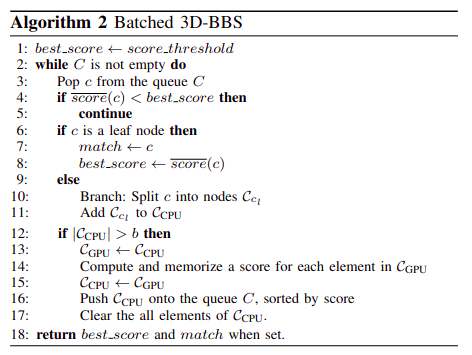
\includegraphics[width=0.75\textwidth]{figures/3dbbs_algorithm.png}
    \caption{3D-BBS Algorithm \cite{aoki20243dbbsgloballocalization3d}}
\end{figure}
\end{frame}


\section{Results}
\label{sec:results}

\subsection{LiDAR Map Generation using KISS-ICP}

A sample LiDAR scan from the KITTI Odometry dataset and the final map generated from 100 scans from the first sequence is demonstrated in \autoref{fig:lidar_scans}. The alignment by KISS-ICP resulted in a absolute trajectory error of 0.082m and an absolute rotational error of 0.061rad.

\begin{figure*}[t]
    \centering
    \begin{subfigure}[t]{0.49\textwidth}
        \centering
        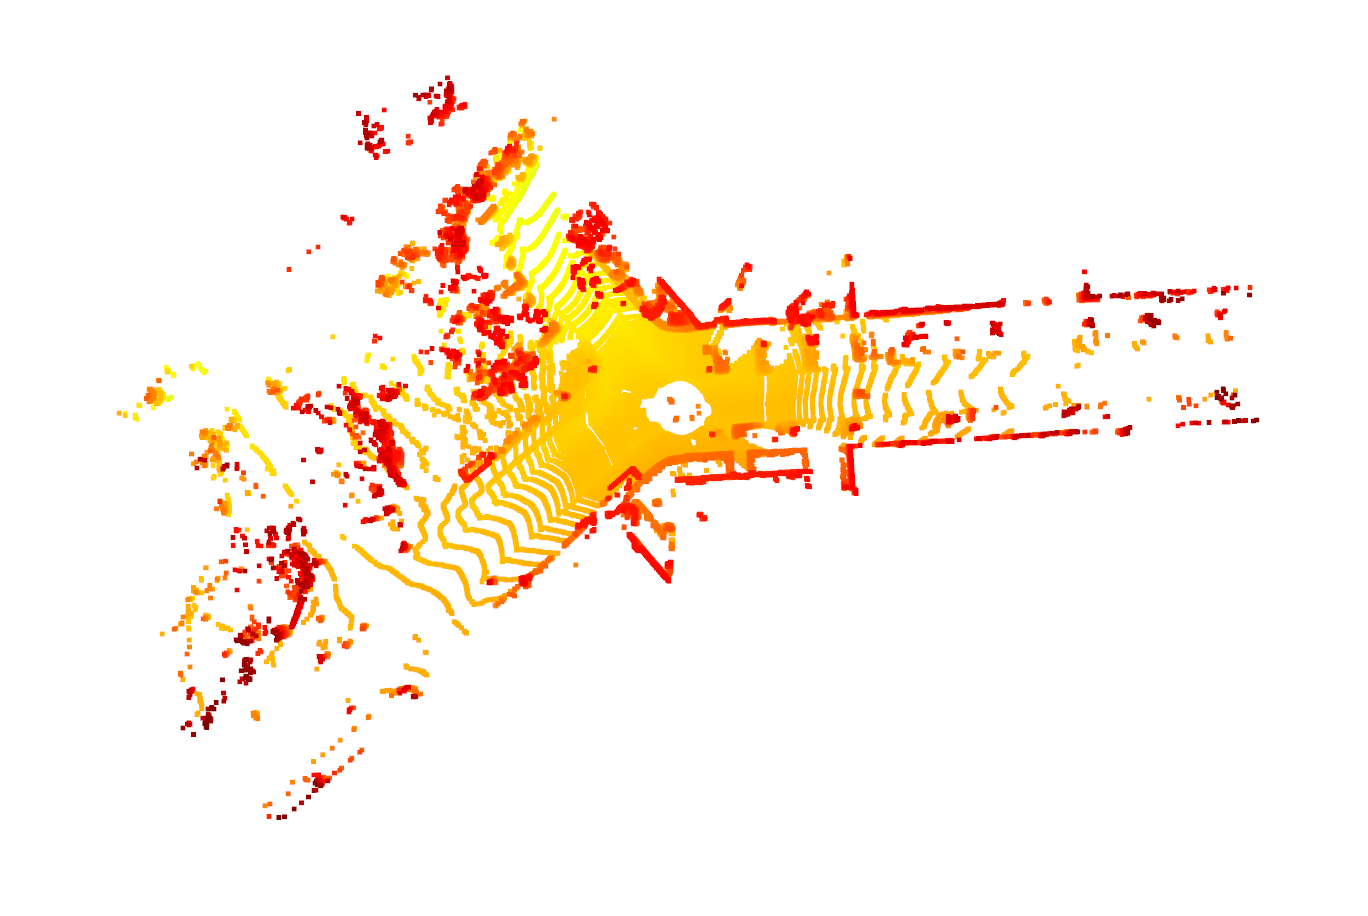
\includegraphics[width=\textwidth]{figures/lidar_frame.png}
        \caption{Sample LiDAR Scan}
    \end{subfigure}
    \begin{subfigure}[t]{0.49\textwidth}
        \centering
        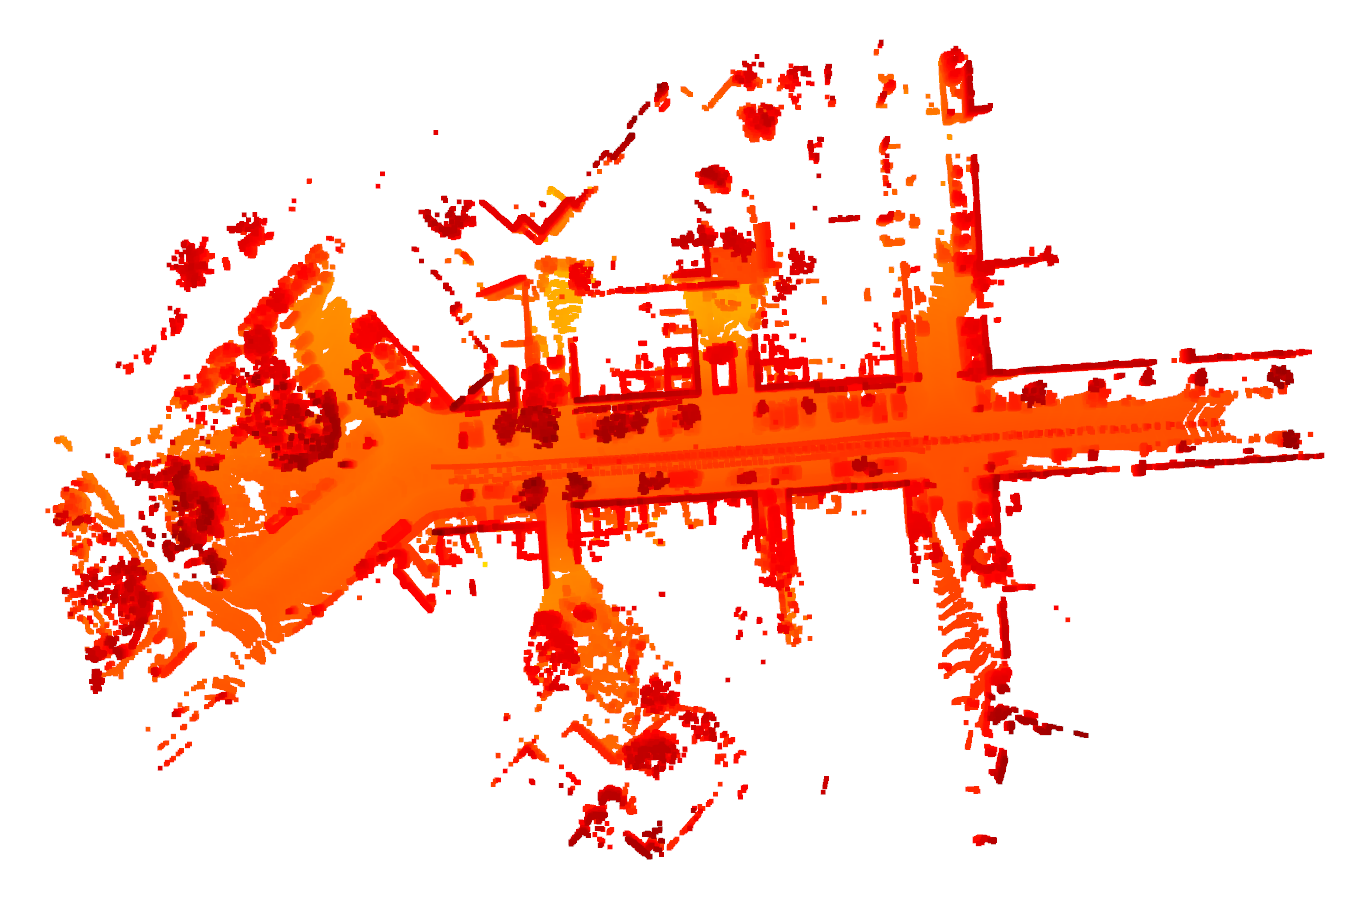
\includegraphics[width=\textwidth]{figures/lidar_map.png}
        \caption{LiDAR Map constructed Using ICP}
    \end{subfigure}
    \caption{Visualization of a sample LiDAR scan and the corresponding LiDAR map constructed using ICP.}
    \label{fig:lidar_scans}
\end{figure*}

\subsection{Ablation Study on 3D-BBS}
The ablation studies reveal the sensitivity of the 3D-BBS algorithm to its configuration parameters, as shown in \autoref{fig:ablation_study}. Increasing \textit{max\_scan\_range}, \textit{min\_level\_res}, and decreasing \textit{src\_leaf\_size} enhances localization accuracy by enabling finer pose subdivisions, reducing translation errors effectively. However, this comes with a trade-off in processing time, as the number of candidate poses increases exponentially with each additional hierarchical level. We did not find any significant pattern with other parameters.

\begin{figure*}[t]
    \centering
    \begin{subfigure}[t]{0.32\textwidth}
        \centering
        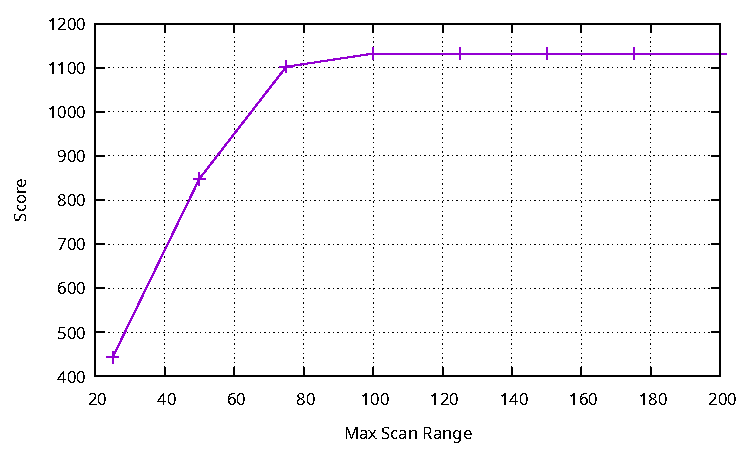
\includegraphics[width=\textwidth]{../02-global-localization/plots/max_scan_range.pdf}
        \caption{Max Scan Range}
    \end{subfigure}
    \begin{subfigure}[t]{0.32\textwidth}
        \centering
        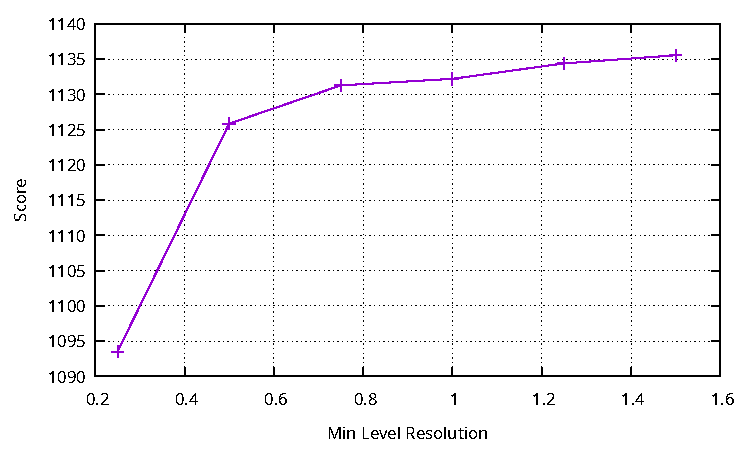
\includegraphics[width=\textwidth]{../02-global-localization/plots/min_level_res.pdf}
        \caption{Min Level Resolution}
    \end{subfigure}
    \begin{subfigure}[t]{0.32\textwidth}
        \centering
        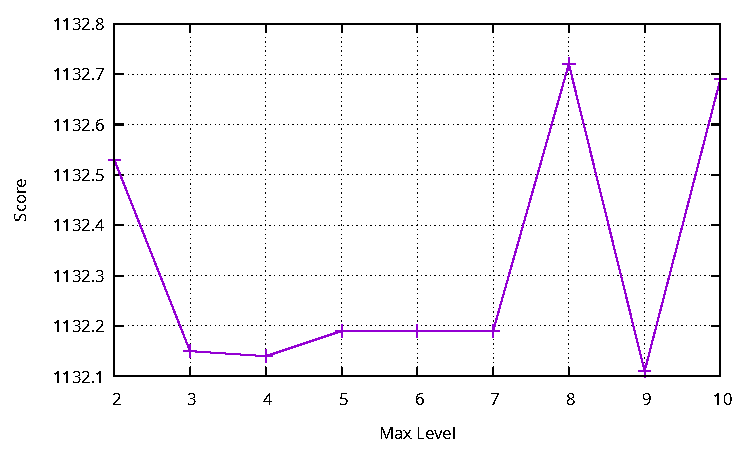
\includegraphics[width=\textwidth]{../02-global-localization/plots/max_level.pdf}
        \caption{Max Level}
    \end{subfigure}
    \begin{subfigure}[t]{0.32\textwidth}
        \centering
        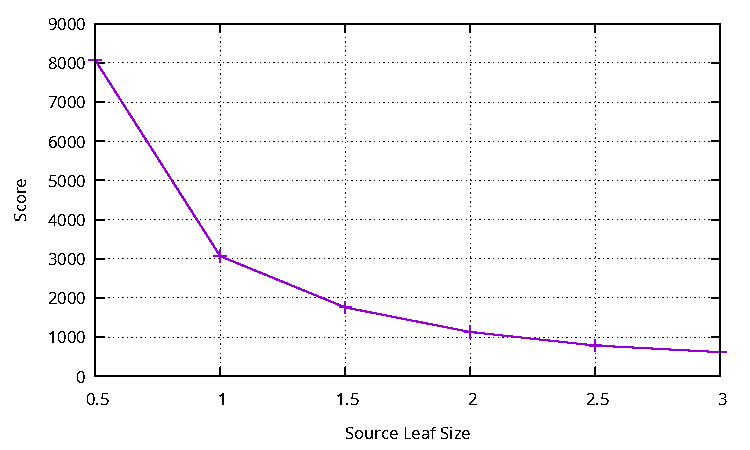
\includegraphics[width=\textwidth]{../02-global-localization/plots/src_leaf_size.pdf}
        \caption{Source Leaf Size}
    \end{subfigure}
    \begin{subfigure}[t]{0.32\textwidth}
        \centering
        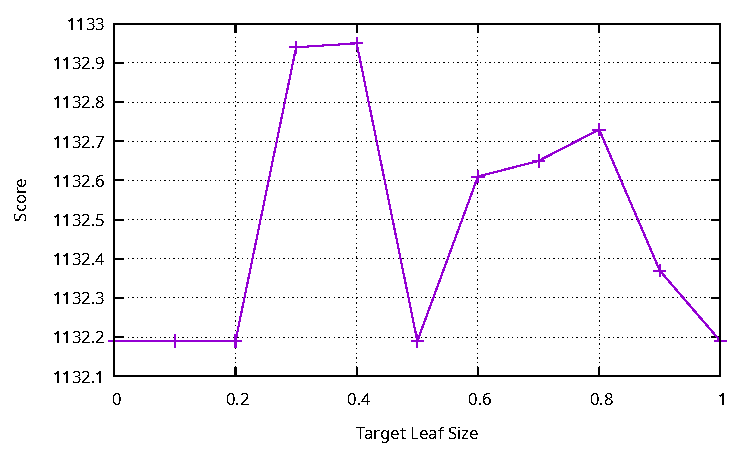
\includegraphics[width=\textwidth]{../02-global-localization/plots/tar_leaf_size.pdf}
        \caption{Target Leaf Size}
    \end{subfigure}
    \caption{Ablation study figures showing change in 3D-BBS localization score with variation in parameters.}
    \label{fig:ablation_study}
\end{figure*}

\subsection{Integration with RGB Images}

A sample RGB image frame from the KITTI Odometry dataset, and the metric depth estimated by Depth Anything v2 is demonstrated in \autoref{fig:image_to_3d_projection}. Note that estimation of metric depth is essential for compatibility of point clouds between different images. We then follow the same procedure with the LiDAR scans to generate a LiDAR map. The resultant map is however not of a very good quality, despite measures such as norm clipping to remove poor estimates of far away points.

\begin{figure*}[t]
    \centering
    \begin{subfigure}[t]{0.49\textwidth}
        \centering
        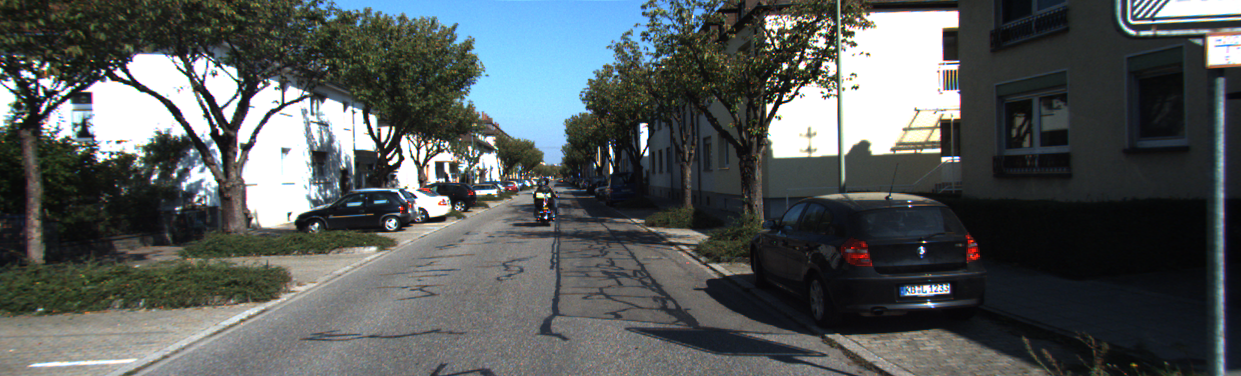
\includegraphics[width=\textwidth]{figures/rgb_image.png}
        \caption{Sample RGB Image}
    \end{subfigure}
    \begin{subfigure}[t]{0.49\textwidth}
        \centering
        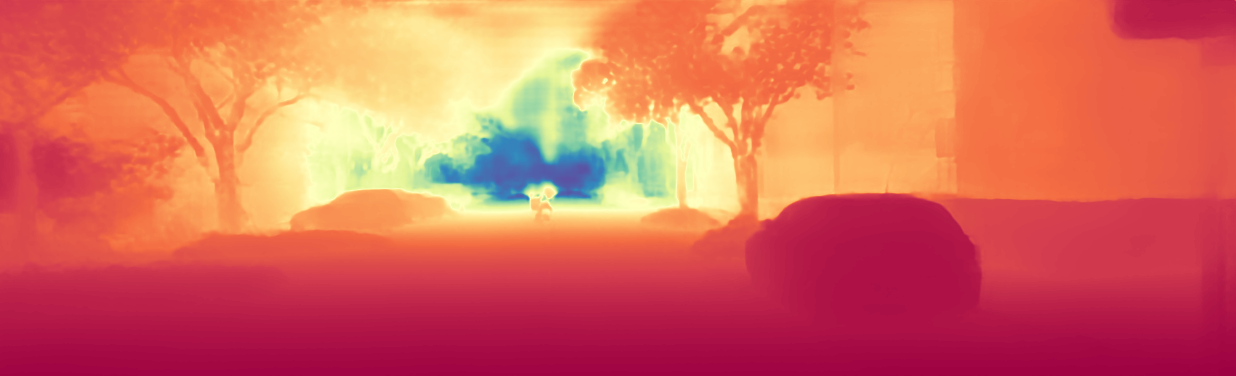
\includegraphics[width=\textwidth]{figures/depth_estimate.png}
        \caption{Metric Depth Estimate}
    \end{subfigure}
    \begin{subfigure}[t]{0.49\textwidth}
        \centering
        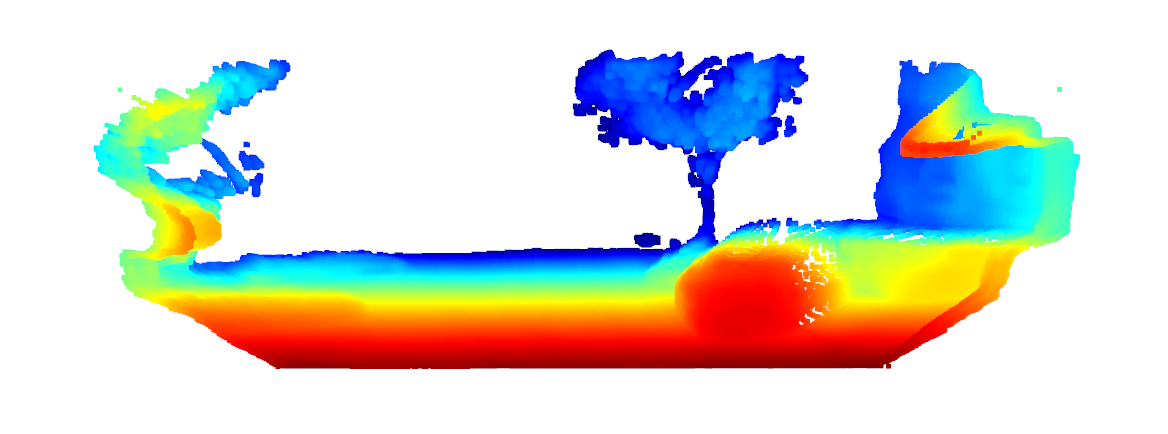
\includegraphics[width=\textwidth]{figures/projected_point_cloud.png}
        \caption{Projected Point Cloud}
    \end{subfigure}
    \begin{subfigure}[t]{0.49\textwidth}
        \centering
        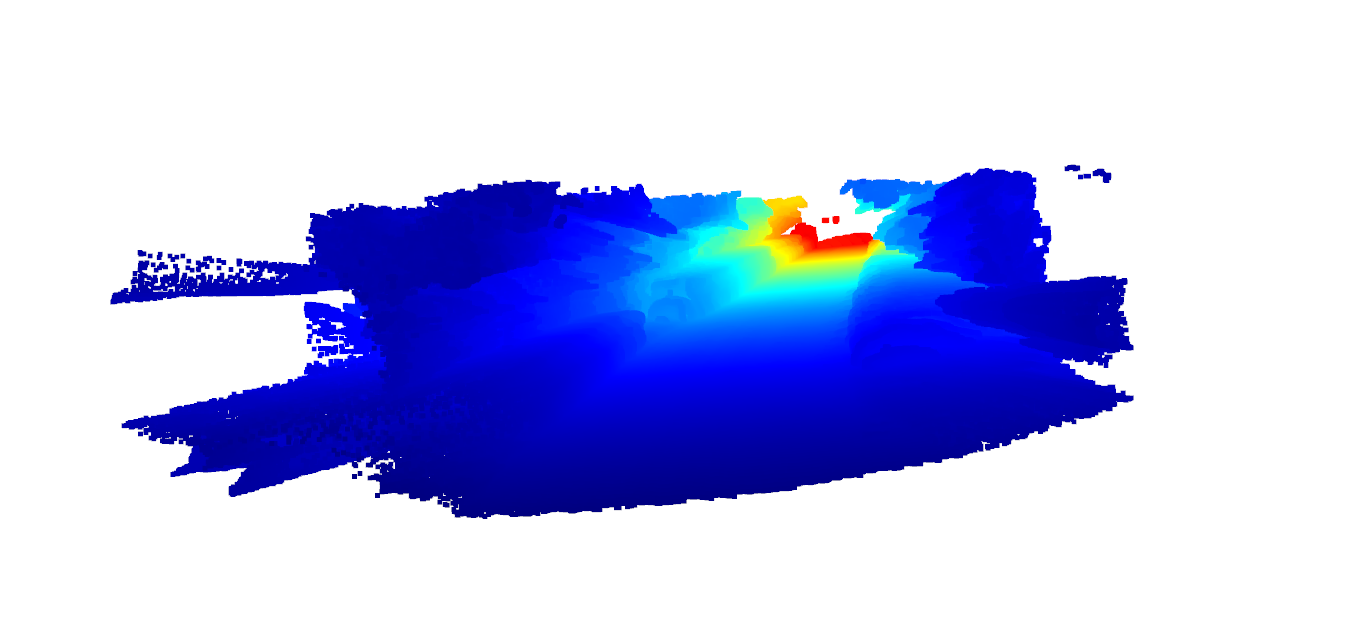
\includegraphics[width=\textwidth]{figures/concatenated_point_cloud.png}
        \caption{Concatenated Point Cloud}
    \end{subfigure}
    \caption{Generation of point cloud by reprojection from the image to 3D space, using depth estimatation.}
    \label{fig:image_to_3d_projection}
\end{figure*}

\subsection{Discussion on 3D-BBS}
The experimental results affirm the efficacy of the 3D-BBS algorithm in achieving accurate and efficient global localization using LiDAR data. The hierarchical BnB approach, combined with sparse voxel mapping and GPU acceleration, addresses the primary challenges associated with 3D localization, including large search spaces and high computational demands.

\subsubsection{Advantages of 3D-BBS}
\begin{itemize}
    \item \textbf{Scalability}: The hierarchical voxel map and sparse representation allow 3D-BBS to scale effectively to large environments without excessive memory consumption.
    \item \textbf{Real-Time Performance}: GPU-accelerated batched processing ensures that localization can be performed within acceptable time frames, making it suitable for real-time applications in autonomous systems.
    \item \textbf{Robustness}: The algorithm maintains high localization accuracy across diverse and dynamic environments, demonstrating resilience against environmental variations and outliers.
    \item \textbf{Flexibility}: The parameter ablation studies provide insights into tuning the algorithm for different scenarios, allowing adaptability to various application requirements.
\end{itemize}

\subsubsection{Limitations and Future Work}
Despite its advantages, the 3D-BBS algorithm has certain limitations that warrant further investigation:

\begin{itemize}
    \item \textbf{Preprocessing Overhead}: The initial voxel map construction is computationally intensive, although it is a one-time cost. Future work could explore incremental map updates to accommodate dynamic environments.
    \item \textbf{Integration with Additional Sensors}: While the integration of RGB images enhances localization, incorporating other sensors such as IMUs or cameras could further improve robustness and accuracy.
    \item \textbf{Adaptive Parameter Tuning}: Developing adaptive mechanisms for parameter tuning based on environmental conditions could enhance the algorithm's flexibility and performance across varied scenarios.
    \item \textbf{Handling Extreme Cases}: Extending the algorithm to handle extreme cases, such as degenerated areas with minimal features or significant occlusions, remains an area for future research.
\end{itemize}


\section{Contributions}
\label{sec:contributions}

The contributions of the authors are as follows:

\begin{enumerate}
    \item \textbf{Himanshu Singh} worked on setting up and integration of the models (KISS-ICP, 3D-BBS and Depth Anything v2) to produce an integrated pipeline, as demonstrated in the results.
    \item \textbf{Pavan Karke} worked on the ablation studies for 3D-BBS.
    \item \textbf{Srinath Bhamidipati} worked on finding the suitable datasets for the project.
\end{enumerate}

\section{Conclusion}
\label{sec:conclusion}

By leveraging a sparse voxel map and integrating roto-translational branching with GPU-accelerated batched processing, 3D-BBS effectively balances localization accuracy with computational efficiency. The ablation studies conducted on key configuration parameters provide valuable insights into optimizing the algorithm for different scenarios, highlighting the importance of scan range, resolution, and point cloud downsampling in achieving optimal performance. Furthermore, the integration of RGB images showcases the potential for multimodal data fusion to enhance localization robustness. Future work can focus on improving the depth estimates of images to generate more accurate point clouds, that can achieve performance comparable to LiDAR scans.


\bibliographystyle{ieeetr}
\bibliography{refs}

\end{document}
